\documentclass[a4paper]{article}

\usepackage{microtype}
\usepackage{fullpage}
\usepackage{mathtools}
\usepackage{amsfonts}
\usepackage{tikz}
\usepackage{pgfplots}
\usepackage{pgfplotstable}
\usepackage{hyperref}
\usepackage[noabbrev,nameinlink]{cleveref}
\usepackage{amsthm}
\usepackage{xcolor}
\usepackage{caption}
\usepackage{subcaption}
\usepackage{setspace}
\usepackage[backend=biber,style=authoryear,maxbibnames=99,hyperref=true]{biblatex} 

\setstretch{1.15}

\addbibresource{src/paper/references.bib}

\usepgfplotslibrary{fillbetween}
\usetikzlibrary{shapes}
\usetikzlibrary{intersections}
\pgfplotsset{compat=1.17}

\newtheorem{definition}{Definition}
\newtheorem{observation}{Observation}
\newtheorem{proposition}{Proposition}
\newtheorem{corollary}{Corollary}
\newtheorem{lemma}{Lemma}
\newtheorem{assumption}{Assumption}

\crefname{assumption}{assumption}{assumptions}
\Crefname{assumption}{Assumption}{Assumptions}
\crefname{observation}{observation}{observations}
\Crefname{observation}{Observation}{Observations}

\newcommand{\dt}{\mathrm{d}t}
\newcommand{\ds}{\mathrm{d}s}
\newcommand{\di}{\mathrm{d}i}
\newcommand{\E}{\mathbb{E}}

\pgfplotstableread[col sep=comma]{out/figures/equilibrium.csv}\equilibrium

\title{Hybrid platforms and bargaining power}
\author{Martin Stancsics}

\begin{document}

\maketitle

\begin{abstract}
    This paper studies the effects of a platform selling their own products in addition to acting as intermediaries (hybrid platforms) in a setting when bargaining takes place between the platform and the potential entrants.
    It highlights a so-far underexplored aspect of hybrid platforms: having their own products increases their bargaining power over the other sellers.
    As shown through a more concrete example, this change in bargaining power can have negative welfare consequences for the consumers.
    The results and methods described in this paper are also applicable to other similar settings, such as vertical integration with a monopolistic upstream supplier.
\end{abstract}


\section{Motivation}

Even though the economics literature offers no unambiguous definition for what platforms are, there seems to be a consensus that they are of key importance for the modern economy, and are getting even more so in the future.
Although market structures resembling various aspects of what we call platforms have existed for some time, the term has only gained widespread usage in the 2000s, with the advent of digitization, and a number of behemoth technology companies playing matchmakers on the internet.
Since then, platforms have become a buzzword in the business world, the subject of increasing regulatory scrutiny, and also a topic of intense academic interest.

Platforms have a number of unique features that make them different from more traditional market structures.
The most prominent of those are multi-sidedness and network effects, which most of the early literature \parencite[for an overview, see][]{rochet2006two} and policy debate \parencite[e.g.][]{fletcher2021consumer,calvano2021market} has focused on.
However, in the more recent years, another important and potentially concerning aspect has been getting more attention: the hybrid operation of certain platforms.
Essentially, this means that platforms act as an intermediary (deciding the rules) and a market participant (competing with other entrants) at the same time.

While hybrid platforms are not a completely new phenomenon, they are becoming more and more common in various industries.
Perhaps the most prominent example is Amazon, which, on the one hand sells its own products, and at the same time hosts ax large number of third-party sellers.
However, examples abound in other industries, as well.
For example, each of the largest digital distribution platforms for computer and smartphone applications (Google Play, Apple App Store and Microsoft Store) sell their own applications besides their third party offerings.
In the video game industry, platform owners studios and publishing games under their own brand is the standard.
Many video streaming services (e.g. Netflix, Amazon Prime Video, Hulu) offer a mix of their own and licensed content.
One can also find examples of similar behavior outside the platform setting, too.
For example BMW is preparing to sell cars directly to consumers in the US, competing with its dealership network.

As deciding the rules of the game and competing in it at the same time gives rise to some obvious concerns, policymakers have been paying increasingly close attention to these platforms in the recent years.
Various pieces of legislation have been proposed to regulate, or even ban e-commerce platforms from selling their own products \parencite[][]{phartiyal_2019,reynolds_2022,eu-2022}.
Furthermore, one of the most prominent ongoing antitrust cases, Microsoft attempting to acquire the video game publisher Activision/Blizzard for a sum of 69 billion USD, is also a case of a platform becoming increasingly hybrid.
This merger would not only increase market concentration on the software side of the video game industry, but might also have further implications for the competition between Microsoft as a platform owner and the other game developers.
The deal is currently under investigation by multiple antitrust authorities, including the US Federal Trade Commission, the European Commission, and the UK Competition and Markets Authority \parencite{livni_merced_2023}.

In parallel to the increasing regulatory interest, the academic literature has also been steadily growing on the topic of hybrid platforms.
\textcite{hagiu2022should} investigate how practices, such as self-preferencing and steering can distort competition on hybrid platforms.
They argue, however, that if such behavior is regulated, the platform selling its own products can be beneficial for consumers.
In contrast to this positive result, \textcite[]{anderson2021hybrid} find that even in the absence of such behavior, allowing hybrid operation might have negative consequences due to platforms having an incentive to exclude competitors from the market.
\textcite[]{gutierrez2021welfare} shows that general conclusions are hard to draw, and welfare effects are platform and product specific.

This paper aims to contribute to this discussion by examining an important, but so far underexplored aspect of platforms: the bargaining power disparity between them and the other market participants, and how this disparity is affected by the platforms' hybrid operation.
In particular, I propose an analytically tractable framework which captures many important aspects of bargaining between one large and a continuum of small players, and apply it to the setting of a hybrid platform facing a continuum of potential entrants.
The results show that, in the presence of bargaining, hybrid operation can indeed have negative welfare consequences for consumers.
This result is particularly striking in this otherwise distortion-free\footnote{
    In the benchmark model without bargaining, the platform's hybrid operation does not affect consumer welfare.
} setting. 
The intuition is that hybrid operation increases the platform's bargaining power against the sntrant sellers.
This in turn leads to a higher entry fee, fewer entrants, then results in lower consumer surplus.
These observations constitute a so-far overlooked aspect of hybrid platforms that policymakers should be aware of.

The closest paper to this one is \textcite{anderson2021hybrid}, which utilizes a similar model and reaches similar conclusions, although through a different mechanism.
I adapt many of the main features of their model with a couple of crucial differences.
Instead of the platform setting a percentage entry fee and being able to commit to it, I assume that (1) platforms charge a lump-sum entry fee and that (2) this entry fee is the result of a negotiation process\footnote{
    The bargaining process is modeled using a solution concept from cooperative game theory, namely the Shapley-value.
    This allows for a tractable analysis while at the same time capturing many of the important features of bargaining.
    Examples of this approach in the industrial organization literature include \textcite{montez2007downstream}, as well as \textcite{hart1990property}, \textcite{levy1997individual}, \textcite{inderst2003bargaining} and \textcite{brugemann2019intra} among others.
}
between the platform and the entrants.
The second point is a novelty not only compared to \textcite{anderson2021hybrid}, but also to the existing literature on hybrid platforms.
Furthermore, in contrast to \textcite{hagiu2022should}, this model is free from any distortive behavior, such as self-preferencing or steering, and the negative results are purely driven by changes in the platform's bargaining position.

This paper is also related to various other strands of the industrial organization literature.
For one, it belongs to the research agenda on understanding platforms and their role in the economy \parencite[e.g.][]{rochet2003platform,hagiu2004optimal,armstrong2006competition,evans2011platform,lee2014competing}.
Furthermore, it is somewhat adjacent to the literature on the importance of exclusive content \parencite[e.g.][]{hagiu2011exclusivity,lee2013vertical,dou2014sell,weeds2016tv}, with the difference that instead of exclusive content giving an advantage against competing platforms, in this paper, own products provide an advantage over entrants.
More generally, many results and concepts of this paper are also applicable outside the context of (multi-sided) platforms.
Certain structures, such as vertical relationships, or even traditional retail stores share a number of features with platforms (notably, the presence of a dominant, indispensable entity), and can be modeled in much the same way.
Therefore, the methodology and results in this paper may also be of interest to researchers studying questions such as retailers having their own private labels \parencite{steiner2004nature} or vertical integration in upstream-downstream markets \parencite{hart1990vertical,aghion2006vertical}.
\textcite{de2005vertical} and \textcite{montez2007downstream}, in which bargaining between the upstream and downstream firms take the center stage, are particularly closely related.

Finally, this paper also belongs to the not too large set of models using concepts from cooperative game theory in an industrial organization setting.
Such examples include the aforementioned \textcite{montez2007downstream}, as well as \textcite{hart1990property}, \textcite{levy1997individual}, \textcite{inderst2003bargaining} and \textcite{brugemann2019intra}, among others.
In contrast to the majority of those, which focus on games with a finite number of players, I utilize an oceanic game (a continuum of small players instead of a finite number), and demonstrate that this can considerably simplify the analysis in certain cases.
Therefore, the modeling approach presented in this paper may be of use in other settings as well.

The rest of the paper is organized as follows.
In \cref{sec:model}, I introduce a general version of the model.
After that, \cref{sec:results} demonstrates results about bargaining outcomes one can derive even in this rather abstract setting.
\Cref{sec:example} concretizes the model by assuming a specific demand system, and also presents a corresponding benchmark model without bargaining.
Finally, \cref{sec:conclusion} summarizes the results and discusses possible future work.


\section{Model}
\label{sec:model}

This section introduces the model used throughout the paper.
I use the terms ``platform'' and ``fringe sellers'', and present my ideas in the context of an intermediated market, such as an online marketplace or an application store.
However, the model is more general, and the results apply to a broader class of settings.
An important example of those is an upstream-downstream setting with a single upstream producer and a continuum of downstream sellers.

Assume that there are two types of players in the market: a platform $P$ and a continuum of fringe sellers $F_i$.
The fringe firms each have one product, which they can only sell through the platform.
The platform itself may also have its own products in addition to acting as an intermediary between the fringe and the consumers.
In that case it is referred to as a hybrid platform.
The main feature of the model is that, instead of assuming that entry fees or royalties are set by the platform and the fringe treat it as take it or leave it offers, I assume that the platform and the fringe engage in some kind of bargaining over their total profits.
The bargaining rule, as well as other details of the model, are described in the rest of this section.


\subsection{Production}

I make use of a reduced-form, but quite general approach to model production and demand.
First, I assume that all fringe firms are ex-ante identical.
This implies that the total profits of the platform and the fringe taken together have a simple functional form $f(n_P, n_F)$.
\begin{assumption}
    \label{ass:identical_fringe}
    The total profits of the platform and the fringe are described by some function $f: \mathbb{R}^+_0 \times \mathbb{R}^+_0 \to \mathbb{R}^+_0$.
\end{assumption}
Here, $n_F$ is the mass of fringe sellers, and $n_P$ measures the degree to which the platform sells its own products.
For example, in a setting with differentiated products and monopolistic competition, $n_F$ and $n_P$ represents the product variety of the fringe and the platform, respectively.
In case the platform operates as a pure intermediary, $n_P = 0$.

I will assume that total profits are increasing in both arguments.
\begin{assumption}
    \label{ass:monotone_profits}
    $f(n_P, n_F)$ is increasing in both $n_P$ and $n_F$.
\end{assumption}
Such profit functions arise in a variety of settings in which the profit reduction from increased competition is dominated by extra sales due to increased variety.
One such example is \textcite{anderson2020aggregative}, where the demand exhibits love for variety, while consumers have access to an outside option.
Alternatively, indirect network effects, such as in two-sided markets, can also result in such profit functions.


\subsection{Profit sharing}

Let us assume that the fringe firms are unable to sell their products directly to consumers.
Instead, they must sell through the platform.
For this service, the platform may charge a fee, and obtain a share of the fringe's profits.

Let us assume that the platform and the fringe shares their total profits according to the following rule.
\begin{assumption}
    \label{ass:profit_sharing}
    Let $w: [0, 1] \to \mathbb{R}_0^+$ such that $\int_0^1 w(s) \ds = 1$. 
    \begin{align*}
        \pi_P(N_P, N_F) &= \int_0^1 w(s) f(N_P, s N_F) \ds, \\
        \pi_F(N_P, N_F) &= f(N_P, N_F) - \int_0^1 w(s) f(N_P, s N_F) \ds.
    \end{align*}
\end{assumption}
While somewhat more complex than a simple percentage split, it has quite a few advantages compared to the latter.\footnote{
    This way of modeling bargaining has precedents in the industrial organization literature \parencite[e.g.][]{hart1990property,segal2003collusion,inderst2003bargaining,montez2007downstream}.
    Furthermore, a number of papers show that various extensive-form bargaining games result in this outcome \parencite{gul1989bargaining,winter1994demand,hart1996bargaining,inderst2003bargaining,stole1996intra}.
}
On the theoretical side, the main argument in favor of this particular rule is its relation to the Shapley-value.\footnote{
    \cref{sec:profit_sharing} shows that in the case of $w(s) \equiv 1$, $\pi_P(N_P, N_F)$ and $\pi_F(N_P, N_F)$ are the Shapely values of the platform and the fringe, respectively.
}
Shapley-value in turn has deep connections to bargaining theory.
\textcite{gul1989bargaining,stole1996intra,hart1996bargaining,inderst2003bargaining}, along with a number of other papers, show that in various extensive-form bargaining games in the players' expected payoffs in the subgame perfect equilibrium correspond to their Shapley values.

The other main justification for this rule its intuitive behavior in terms of comparative statistics when varying $f$ and $w$.
To illustrate this, let us examine the various parts of this rule, and then discuss how they impact the platform's profit share.

The main feature of this rule is that the platform's bargaining power depends on the degree to which the fringe firms are complements or substitutes of each other.
The following observation demonstrates this idea.
\begin{observation}
    \label{prop:outcome_based_bargaining_power}
    Fix some $N_P \geq 0$. Let $f, \tilde{f}: \mathbb{R}^+_0 \times \mathbb{R}^+_0 \to \mathbb{R}^+_0$ two different total profit functions such that $f(N_P, N_F) = \tilde{f}(N_P, N_F)$ for some $N_P, N_F$ and $f(N_P, n_F) \leq \tilde{f}(N_P, n_F)$ for all $n_F < N_F$.
    Furthermore, let us denote the corresponding platform profit shares by $\pi_P$ and $\tilde{\pi}_P$.
    
    Then, $\pi_P \leq \tilde{\pi}_P$.
\end{observation}

In words, \cref{prop:outcome_based_bargaining_power} describes two alternative profit functions, under which $N_F$ fringe firms (along with the platform and it's $N_P$ products) are able to achieve the same total profit level.
However, in one of these cases, the fringe firms are more substitutable to each other, in the sense that fewer of them are needed to achieve a given level of profit (see \cref{fig:outcome_based_bargaining_power}).
The observation is that, in this situation, the platform's share is indeed higher when the fringe firms are more substitutable.
This coincides with the intuitive idea that the platform's bargaining power is higher when it does not really mind loosing a few fringe sellers.

\begin{figure}
    \centering
    \begin{subfigure}[b]{0.45\textwidth}
        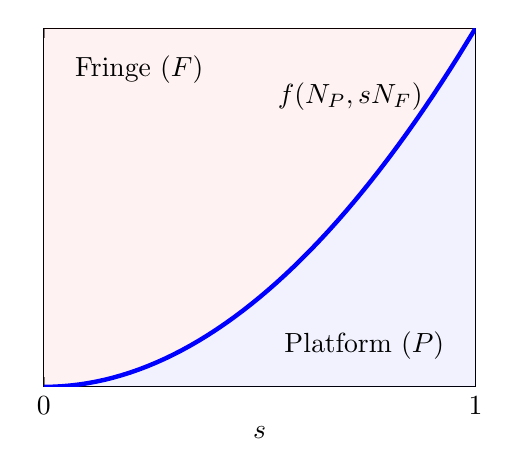
\begin{tikzpicture}[scale=0.8]
            \centering
            \begin{axis}[xmin=0, xmax=1, ymin=0, ymax=1, samples at={0, 0.02, ..., 0.98, 1},
                    xtick={0, 1}, ytick=\empty, xlabel={$s$}]
                \addplot[name path=f, blue,ultra thick] {x^2};
                \node[anchor= east] at (axis cs: .9, .9^2) {$f(N_P, sN_F)$};
                \path[name path=bottom] (axis cs:0,0) -- (axis cs:1,0);
                \path[name path=top] (axis cs:0,1) -- (axis cs:1,1);
    
                \addplot [fill=blue, fill opacity=0.05] fill between [of=f and bottom];
                \addplot [fill=red, fill opacity=0.05] fill between [of=f and top];
    
                \node[anchor=north west] at (axis cs: .05, .95) {Fringe ($F$)};
                \node[anchor=south east] at (axis cs: .95, .05) {Platform ($P$)};
            \end{axis}
        \end{tikzpicture}
        \caption{Fringe firms are complements}
    \end{subfigure}
    \begin{subfigure}[b]{0.45\textwidth}
        \centering
        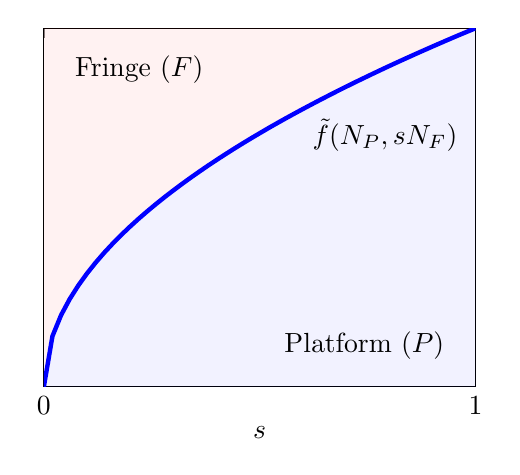
\begin{tikzpicture}[scale=0.8]
            \begin{axis}[xmin=0, xmax=1, ymin=0, ymax=1, samples at={0, 0.02, ..., 0.98, 1},
                xtick={0, 1}, ytick=\empty, xlabel={$s$}]
                \addplot[name path=f, blue,ultra thick] {x^0.5};
                \node[anchor=north west] at (axis cs: .6, .6^0.5) {$\tilde{f}(N_P, sN_F)$};
                \path[name path=bottom] (axis cs:0,0) -- (axis cs:1,0);
                \path[name path=top] (axis cs:0,1) -- (axis cs:1,1);
    
                \addplot [fill=blue, fill opacity=0.05] fill between [of=f and bottom];
                \addplot [fill=red, fill opacity=0.05] fill between [of=f and top];
    
                \node[anchor=north west] at (axis cs: .05, .95) {Fringe ($F$)};
                \node[anchor=south east] at (axis cs: .95, .05) {Platform ($P$)};
            \end{axis}
        \end{tikzpicture}
        \caption{Fringe firms are substitutes}
    \end{subfigure}
    \caption{Distribution of value between the platform and the fringe (with $w(s) \equiv 1$)}
    \label{fig:outcome_based_bargaining_power}
\end{figure}


The other main ingredient of the sharing rule, $w(s)$, captures the platform's \emph{innate} bargaining power.
It is independent of the production function, demand, or the fringe firms' substitutability, and might represent, for example, that the platform and the fringe firms have different power to propose allocations during the (not explicitly modeled) negotiation process.\footnote{
    For a more thorough exploration of this idea, see \textcite{hart1996bargaining}.
}

One way to think about the weighting is that the platform's share is the expectation of the total profit, when the number of fringe firms is drawn from $[0, N_F]$ according to some distribution.\footnote{
    In fact, this is exactly the idea behind the Shapley value: the platform (and other players, too) gets its expected marginal contribution to the total profit.
    As the fringe cannot create any value without the platform, the latter's marginal contribution to a coalition of $n_F$ fringe firms is simply $f(n_F)$.
}
An obvious choice is to use the uniform distribution, in which case the shares correspond to the Shapley value.
However, this is not the only possible choice.
If, for example, we want to assume that the platform has a higher innate bargaining power, we can use a distribution with a higher mass on the right tail.\footnote{
    Specific choices for $w$ can also be motivated by cooperative game theoretical concepts.
    For example using, $w(s) = \lambda t^{\lambda - 1}$ leads to the weighted Shapley value, with weights $\lambda$ and $1$ for the platform and the fringe firms, respectively.
}
When the distribution $W_1$ first order stochastically dominates another distribution $W_2$, the platform is more likely to draw a value from with a higher mass of fringe firms, and therefore obtain a higher profit share in case of $W_1$ than in the case of $W_2$.
The next observation formalizes this idea.
\begin{observation}
    \label{prop:innate_bargaining_power}
    Let $w, \tilde{w}: [0, 1] \to \mathbb{R}_0^+$ be two different weight functions such that $\int_0^x w_1(s) \ds \leq \int_0^x w_2(s) \ds$ for all $x \in [0, 1]$.
    As before, let us denote the corresponding platform profit shares by $\pi_P$ and $\tilde{\pi}_P$.
    
    Then, $\pi_P(N_P, N_F) \leq \tilde{\pi}_P(N_P, N_F) \; \forall\, N_P \geq 0, N_F > 0$.
    Furthermore, this inequality is strict if $\int_0^x w_1(s) \ds < \int_0^x w_2(s) \ds$ on some non-zero measure set.
\end{observation}

Although the reasoning is straightforward, it establishes that $w$ can indeed be used to represent some form of innate bargaining power.
For example, if one has reason to believe that the platform has a stronger voice in the negotiation process, one can use a weight function with a higher mass on larger values.


\subsection{Entry and equilibrium}

Let us now turn to the determination of the equilibrium number of fringe firms.
Assume that there is an unlimited number of potential fringe entrants, indexed by $i \in \mathbb{R}^+_0$.
In the first stage of the game, each fringe firm must create a viable product at the investment cost $I_F > 0$.
In the second stage, firms that made this investment plus the platform engage in producing and selling their respective products.
If there are $N_F$ fringe entrants and $N_P$ platform products, then, as discussed previously, the total profit they make together is given by $f(N_P, N_F)$.
Finally, the platform and the entrants share this profit according to the profit sharing rule from \cref{ass:profit_sharing}.

The equilibrium number of entrants is determined by a free entry condition: in the end, the fringe firms' profits should be equal to the investment cost.
\begin{definition}
    \label{ass:free_entry}
    Let us define a free entry equilibrium by the following conditions:
    \begin{itemize}
        \item Profits are shared according to \cref{ass:profit_sharing}.
        \item Entrants make zero profits: $\pi_F(N_P, N_F) = I_F N_F$ after accounting for entry costs.
    \end{itemize}
\end{definition}

Finally, in order to guarantee a unique equilibrium, let us make the following, an additional assumption about the profit and bargaining weight functions.
\begin{assumption}
    \label{ass:single_crossing}
    Let $f$ and $w$ be such that the following holds for all $N_F, N_P \geq 0$:
    \begin{gather*}
        f'_{n_F} (N_P, N_F) < \int_0^1 s w(s) f'_{n_F} (N_P, s N_F) \ds \\
        \text{or} \\
        f''_{n_F} (N_P, N_F) < \int_0^1 s^2 w(s) f''_{n_F} (N_P, s N_F) \ds.
    \end{gather*}
\end{assumption}
The above assumption essentially guarantees that the profit of the fringe (as a function of the number of entrants) has at most a single crossing with the total entry cost (apart from the obvious $N_F=0$ intersection).
While the conditions is not very simple to interpret, they can be verified once a specific choice for $f$ and $w$ is made.
In particular, this assumption will be satisfied in the example in \cref{sec:example}.


\section{General results}
\label{sec:results}

This section presents some general result that only depend on the abstract model structure described in the previous section, and the assumptions therein.
It is remarkable that even within such a stylized setting and simple model, one can derive some interesting and non-trivial results.
\Cref{sec:example} will then build on these results to derive some stronger implications in a more specific model.

Let us start by a technical, but highly useful result.
\begin{proposition}
    \label{prop:unique_equilibrium}
    Under the conditions in \cref{ass:single_crossing}, the equilibrium is unique if it exists.
\end{proposition}
The intuition behind this result is that \cref{ass:single_crossing} ensures that the total profits achieved by the fringe is either concave or hump-shaped.
Consequently, it has at most one crossing with the linear total entry cost (for $n_F > 0$).
An example for this is shown in \cref{fig:equilibrium}.
This particular shape is also the main driver for the following results about the comparative statics of equilibrium profits and entry.

\begin{figure}[ht]
    \centering
    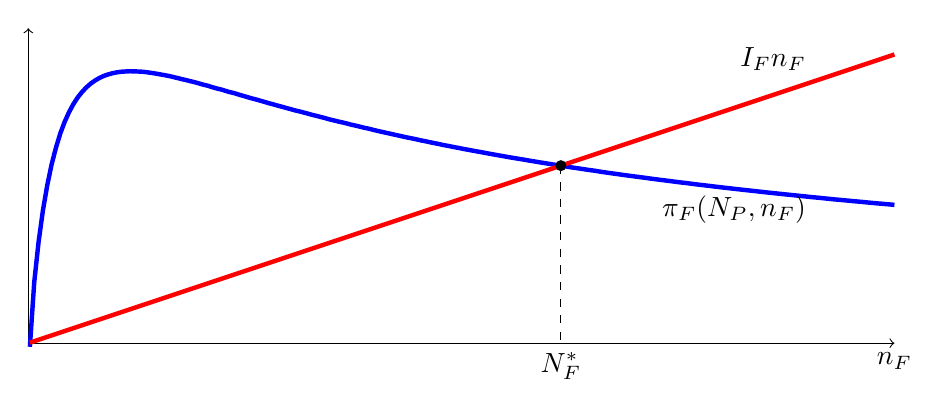
\begin{tikzpicture}[xscale=2,yscale=2,samples=200]
        \draw[->] (0,0) -- (0,2);
        \draw[->] (0,0) -- (5.5,0) node[below] {$n_F$};

        \draw[name path=piF,domain=0.01:5.5,variable=\x,blue,ultra thick] plot ({\x},{8*((\x)/(0.3+\x))-8*((\x-0.3*ln(\x+0.3)-0.361)/(\x))});
        \draw[name path=IF,domain=0.01:5.5,variable=\x,red,ultra thick] plot ({\x},{(\x)/3});
        \node[anchor=north east] at (5,1) {$\pi_F(N_P, n_F)$};
        \node[anchor=south east] at (5,5/3) {$I_F n_F$};

        \fill [name intersections={of=piF and IF, name=i, total=\t}]
            [black] (i-2) circle (1pt);
        \draw[dashed] (i-2) -- (i-2 |- 0,0) node[below] {$N_F^*$};
    \end{tikzpicture}
    \caption{An example free entry equilibrium under \cref{ass:single_crossing}}
    \label{fig:equilibrium}
\end{figure}

For the following two propositions, let us ignore free entry and equilibrium behavior, and consider the number of fringe entrants $N_F$ as fixed.
The following statement says that the platform's profit is increasing in its own product variety.
\begin{proposition}
    \label{prop:share_of_platform}
    Assume that $f$ is continuously differentiable with respect to $N_P$ and also twice differentiable.
    Let $N_F \geq 0$.
    Then $\pi_P$ is also differentiable and
    $$\frac{\partial \pi_P(N_P, N_F)}{\partial N_P} > 0$$.
\end{proposition}
While it might seem obvious, let us still examine what this result does and does not mean.
First, remember that $f$ is increasing in both arguments, and $N_F$ is fixed.
Therefore, an increase in $N_P$ also increases the size of the pie the participants bargain over.
This result states that the size of the pie that the platform gets increases in this case, too.
It does not mean, however, that the \emph{relative share} of the pie that the platform gets is also bigger -- increase is also guaranteed in absolute terms.
For example, it is possible that for the new, higher value of $N_P$, the complementarities between the fringe firms become stronger, and the platform's bargaining power decreases.
This decrease cannot be so strong, however, to decrease the platform's profits in absolute terms.
\cref{fig:increase_N_P_platform} shows an example of this situation.

\begin{figure}[ht]
    \centering
    \begin{subfigure}[b]{0.45\textwidth}
        \centering
        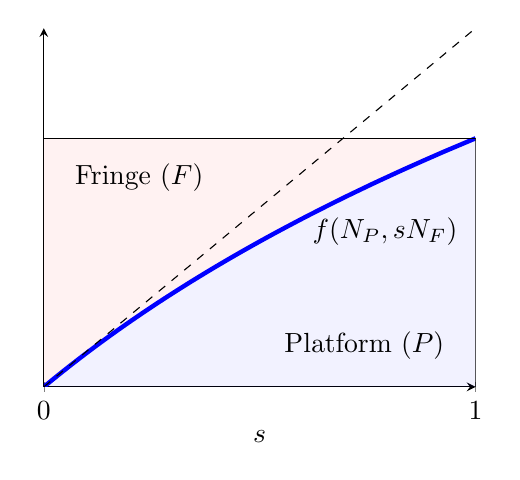
\begin{tikzpicture}[scale=0.8]
            \begin{axis}[xmin=0, xmax=1, ymin=0, ymax=1, samples at={0, 0.02, ..., 0.98, 1},
                xtick={0, 1}, ytick=\empty, axis lines=left, xlabel={$s$}]
                \addplot[name path=f, blue,ultra thick] {ln(1+x)};
                \addplot[name path=tildef, dashed, black] {x};
                \node[anchor=north west] at (axis cs: .6, 0.5) {$f(N_P, sN_F)$};
                \path[name path=bottom] (axis cs:0,0) -- (axis cs:1,0);
                \draw[name path=top] (axis cs:0,0.693) -- (axis cs:1,0.693);
                \draw[name path=right] (axis cs:1,0) -- (axis cs:1,0.693);
    
                \addplot [fill=blue, fill opacity=0.05] fill between [of=f and bottom];
                \addplot [fill=red, fill opacity=0.05] fill between [of=f and top];
    
                \node[anchor=north west] at (axis cs: .05, .65) {Fringe ($F$)};
                \node[anchor=south east] at (axis cs: .95, .05) {Platform ($P$)};
            \end{axis}
        \end{tikzpicture}
        \caption{Profit shares with $N_P$}
    \end{subfigure}
    \begin{subfigure}[b]{0.45\textwidth}
        \centering
        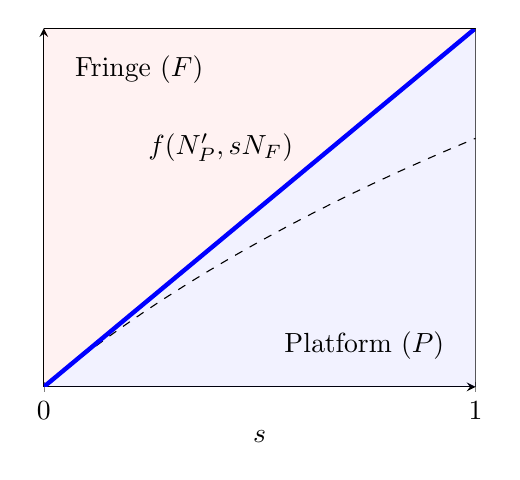
\begin{tikzpicture}[scale=0.8]
            \begin{axis}[xmin=0, xmax=1, ymin=0, ymax=1, samples at={0, 0.02, ..., 0.98, 1},
                xtick={0, 1}, ytick=\empty, axis lines=left, xlabel={$s$}]
                \addplot[name path=f, dashed, black] {ln(1+x)};
                \addplot[name path=tildef, blue,ultra thick] {x};
                \node[anchor=south east] at (axis cs: 0.6, 0.6) {$f(N_P', sN_F)$};
                \path[name path=bottom] (axis cs:0,0) -- (axis cs:1,0);
                \draw[name path=top] (axis cs:0,1) -- (axis cs:1,1);
                \draw[name path=right] (axis cs:1,0) -- (axis cs:1,1);
    
                \addplot [fill=blue, fill opacity=0.05] fill between [of=tildef and bottom];
                \addplot [fill=red, fill opacity=0.05] fill between [of=tildef and top];
    
                \node[anchor=north west] at (axis cs: .05, .95) {Fringe ($F$)};
                \node[anchor=south east] at (axis cs: .95, .05) {Platform ($P$)};
            \end{axis}
        \end{tikzpicture}
        \caption{Profit shares with $N_P'$}
    \end{subfigure}
    \caption{Illustration of \cref{prop:share_of_platform} ($N_P < N_P'$)}
    \label{fig:increase_N_P_platform}
\end{figure}

Next, let us look at an analogous result for the fringe firms.
As the next proposition demonstrates, in this case, the direction of the change depends on the complementarities between the fringe firms.
\begin{proposition}
    \label{prop:share_of_fringe}
    Assume that $f, w$ are twice continuously differentiable.
    Let $N_F > 0$.
    Then $\pi_F$ is also differentiable.
    \begin{align*}
        &\text{If } \frac{\partial^2 f(N_P, n_F)}{\partial n_P \partial n_F} < 0 \;\forall n_F \leq N_F, \text{ then } \frac{\partial \pi_F(N_P, N_F)}{\partial N_P} < 0, \\
        &\text{if } \frac{\partial^2 f(N_P, n_F)}{\partial n_P \partial n_F} > 0 \;\forall n_F \leq N_F, \text{ then } \frac{\partial \pi_F(N_P, N_F)}{\partial N_P} > 0
    \end{align*}
    for all $N_P \geq 0$.
\end{proposition}
In summary, when they are mostly substitutes (the cross-derivatives of $f$ are negative), the fringe's profits decrease as a result of an increase in $N_F$.
The intuition is that, even though the total size of the pie increases, the bargaining power of the fringe deteriorates so much that its share decreases not only in relative, but also in absolute terms (as illustrated in \cref{fig:increase_N_P_fringe}).
On the other hand, when the fringe firms are mostly complements the fringe's profits increase.

\begin{figure}[ht]
    \centering
    \begin{subfigure}[b]{0.45\textwidth}
        \centering
        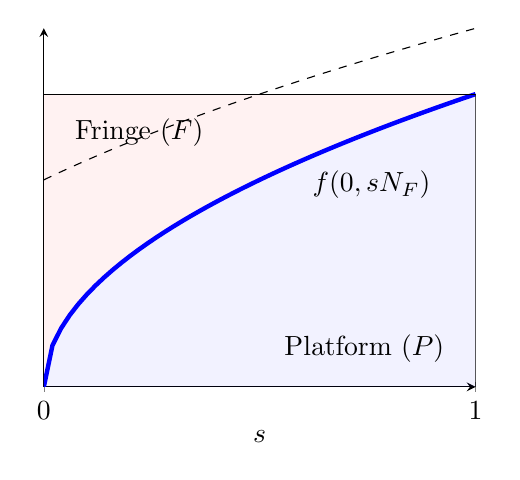
\begin{tikzpicture}[scale=0.8]
            \begin{axis}[xmin=0, xmax=1, ymin=0, ymax=1.225, samples at={0, 0.02, ..., 0.98, 1},
                xtick={0, 1}, ytick=\empty, axis lines=left, xlabel={$s$}]
                \addplot[name path=f, blue,ultra thick] {sqrt(x)};
                \addplot[name path=tildef, dashed, black] {sqrt(0.5+x)};
                \node[anchor=north west] at (axis cs: .6, 0.77) {$f(0, sN_F)$};
                \path[name path=bottom] (axis cs:0,0) -- (axis cs:1,0);
                \draw[name path=top] (axis cs:0,1) -- (axis cs:1,1);
                \draw[name path=right] (axis cs:1,0) -- (axis cs:1,1);
    
                \addplot [fill=blue, fill opacity=0.05] fill between [of=f and bottom];
                \addplot [fill=red, fill opacity=0.05] fill between [of=f and top];
    
                \node[anchor=north west] at (axis cs: .05, .95) {Fringe ($F$)};
                \node[anchor=south east] at (axis cs: .95, .05) {Platform ($P$)};
            \end{axis}
        \end{tikzpicture}
        \caption{Profit shares with $N_P = 0$}
    \end{subfigure}
    \begin{subfigure}[b]{0.45\textwidth}
        \centering
        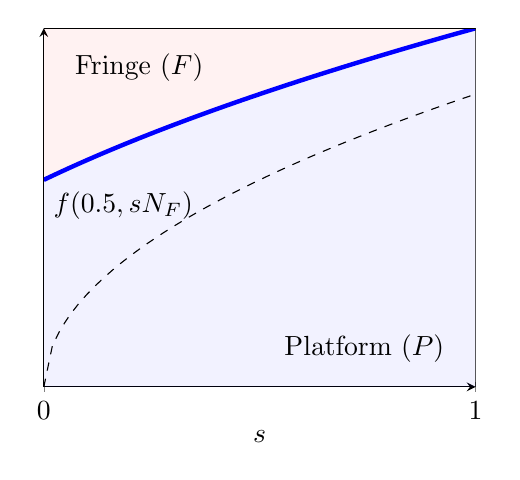
\begin{tikzpicture}[scale=0.8]
            \begin{axis}[xmin=0, xmax=1, ymin=0, ymax=1.225, samples at={0, 0.02, ..., 0.98, 1},
                xtick={0, 1}, ytick=\empty, axis lines=left, xlabel={$s$}]
                \addplot[name path=f, dashed, black] {sqrt(x)};
                \addplot[name path=tildef, blue,ultra thick] {sqrt(0.5+x)};
                \node[anchor=north west] at (axis cs: 0, 0.7) {$f(0.5, sN_F)$};
                \path[name path=bottom] (axis cs:0,0) -- (axis cs:1,0);
                \draw[name path=top] (axis cs:0,1.225) -- (axis cs:1,1.225);
                \draw[name path=right] (axis cs:1,0) -- (axis cs:1,1.225);
    
                \addplot [fill=blue, fill opacity=0.05] fill between [of=tildef and bottom];
                \addplot [fill=red, fill opacity=0.05] fill between [of=tildef and top];
    
                \node[anchor=north west] at (axis cs: .05, 1.17) {Fringe ($F$)};
                \node[anchor=south east] at (axis cs: .95, .05) {Platform ($P$)};
            \end{axis}
        \end{tikzpicture}
        \caption{Profit shares with $N_P = 0.5$}
    \end{subfigure}
    \caption{Illustration of \cref{prop:share_of_fringe} (fringe firms are substitutes, $f(N_P, N_F) = \sqrt{N_P + N_F}$)}
    \label{fig:increase_N_P_fringe}
\end{figure}

Now let us turn to equilibrium entry as a function of the platform's product variety.
The previous proposition implies an almost immediate corollary regarding the equilibrium number of fringe entrants.
\begin{corollary}
    \label{cor:fringe_entry}
    Assume that $f, w$ are twice continuously differentiable.
    Let $N_F^*$ denote the equilibrium number of fringe firms.
    Let us also assume that $N_F^* > 0$.
    Furthermore, let us assume that
    \begin{align*}
        \frac{\partial^2 f(n_P, n_F)}{\partial n_P \partial n_F} < 0 \quad \forall n_F \leq N_F \\
        \frac{\partial^2 f(n_P, n_F)}{\partial n_F^2} < 0 \quad \forall n_F \leq N_F.
    \end{align*}
    Then the equilibrium number of fringe firms is also differentiable and
    \begin{align*}
        \frac{\partial N_F^*}{\partial N_P} < 0.
    \end{align*}
\end{corollary}
That is, the equilibrium number of entrants increases as a response to an increase in $N_P$ if the fringe firms are mostly complements, and decreases if they are mostly substitutes.
The reason simply lies in the concave or hump-shaped fringe profit function.
If $N_F^*$ is an equilibrium, then fringe profits minus entry costs are strictly positive for all $N_F \leq N_F^*$ and strictly negative for all $N_F > N_F^*$.
Therefore, if an increase in $N_P$ decreases the fringe's profits for every $N_F \geq 0$, equilibrium can be restored by decreasing the number of fringe entrants, and vice versa for the other case (\cref{fig:comparative_N_F}).

\begin{figure}[ht]
    \centering
    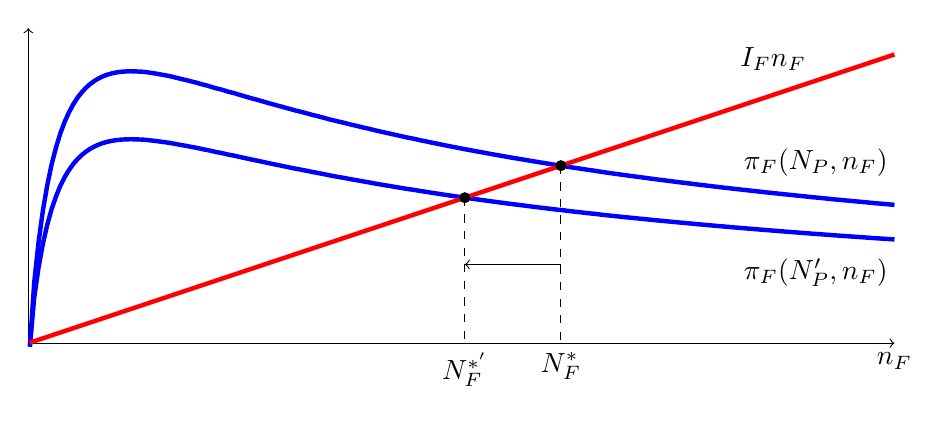
\begin{tikzpicture}[xscale=2,yscale=2,samples=200]
        \draw[->] (0,0) -- (0,2);
        \draw[->] (0,0) -- (5.5,0) node[below] {$n_F$};

        \draw[name path=piF,domain=0.01:5.5,variable=\x,blue,ultra thick] plot ({\x},{8*((\x)/(0.3+\x))-8*((\x-0.3*ln(\x+0.3)-0.361)/(\x))});
        \draw[name path=piF2,domain=0.01:5.5,variable=\x,blue,ultra thick] plot ({\x},{6*((\x)/(0.3+\x))-6*((\x-0.3*ln(\x+0.3)-0.361)/(\x))});
        \draw[name path=IF,domain=0.01:5.5,variable=\x,red,ultra thick] plot ({\x},{(\x)/3});

        \node[anchor=south] at (5,1) {$\pi_F(N_P, n_F)$};
        \node[anchor=north] at (5,0.6) {$\pi_F(N_P', n_F)$};
        \node[anchor=south east] at (5,5/3) {$I_F n_F$};

        \fill [name intersections={of=piF and IF, name=i, total=\t}]
            [black] (i-2) circle (1pt);
        \draw[dashed] (i-2) -- (i-2 |- 0,0) node[below] {$N_F^*$};
        \fill [name intersections={of=piF2 and IF, name=i2, total=\t}]
            [black] (i2-2) circle (1pt);
        \draw[dashed] (i2-2) -- (i2-2 |- 0,0) node[below] {$N_F^{*'}$};

        \draw[->] (i-2 |- 0,0.5) -- (i2-2 |- 0,0.5);
    \end{tikzpicture}
    \caption{Illustration of comparative statics for equilibrium entry}
    \label{fig:comparative_N_F}
\end{figure}

Finally, let us conclude this section by establishing a stronger result for a more restrictive class of profit functions.
In the following, I assume that the profit function has a specific, additive form.
Intuitively, this means that -- in terms of total profits generated -- the platform's and the fringe firms' products are substitutable to each other according to some constant ratio.\footnote{
    Note that it does not mean that their products are substitutes in the usual, demand theory sense.
    They still might be complements to each other.
}
\begin{proposition}
    \label{prop:aggregate_size_additive}
    Let the weight function be constant ($w(t) \equiv 1$).
    % TODO: I think the weight function assumption is not necessary.
    Furthermore, let $f$ have the following, additive form:
    \begin{align*}
        f(N_P, N_F) = g(\alpha N_P + \beta N_F)
    \end{align*}
    where $\alpha, \beta > 0$.
    Also assume that $g$ is twice differentiable and that $g'' < 0$.
    Then
    \begin{align*}
        \frac{\partial N_F^*}{\partial N_P} < -\frac{\alpha}{\beta}.
    \end{align*}
\end{proposition}
As opposed to the previous results, this proposition tells us something about the total profits generated by the platform and the fringe firms as a function of the platform's product variety, and under equilibrium entry behavior by the fringe firms.
In particular, it states that total profits increase if the total profit function is convex (products are substitutes), and decreases otherwise.
This result has particularly strong implications in models where total profits (or total product variety) has a monotone relationship with consumer welfare, such as those in \textcite{anderson2020aggregative}.
\Cref{sec:example} also presents a model in which this is the case.


\section{Example application}
\label{sec:example}

Let us now turn to an example application of the somewhat abstract model presented in the previous sections.
The model in this section is heavily inspired by the logit-like demand structure and hybrid platform setting in  \textcite{anderson2021hybrid}.
The setting is a (possibly hybrid) platform market with monopolistically competing fringe firms.

\subsection{Setup}

\subsubsection{Demand}

Imagine that there is a unit mass of consumers, looking to buy one product each.
They choose from a continuum of products, indexed by $i$.
Customer $j$ derives the following utility from buying product $i$:
\begin{align*}
    u^F_{ij} = v^F_i - p^F_i + \mu\epsilon^F_{ij},
\end{align*}
where $v^F_i$ is the value of product $i$, $p^F_i$ is its price, and $\epsilon^F_{ij}$ is an idiosyncratic taste shock.
Throughout this section I assume that the value of each product is the same: $v^F_i = v^F$.
This is to simplify the analysis, but is not crucial for getting the results.  % TODO: look into relaxing this assumption

Additionally, customers can also choose from a unit mass of outside options, yielding utility $u^0_ij = \mu\epsilon^0_{ij}$. $\epsilon^F_{ij}$ and $\epsilon^0_{ij}$ are assumed to be independent and identically distributed (i.i.d.) across consumers and products, and follow a standardized Type I Extreme Value distribution. This distributional assumption, along with the fact that each consumer consumes only one product, will lead to a tractable, logit-form demand function.

\subsubsection{Production}

Each (horizontally differentiated) product is produced by a single, monopolistically competitive (fringe) seller.
The production entails a constant marginal cost $c^F_i$.
As with the value, I assume that the marginal cost is the same for all products: $c^F_i = c^F$.
Facing the demand described in the previous paragraphs, the sellers choose their price $p^F_i$ to maximize profits.

Additionally, the platform itself can also offer mass $N_P$ of its own products.
The value and marginal cost of these products are denoted by $v^P$ and $c^P$, respectively.
Furthermore, consumers have the same i.i.d. taste shocks ($\epsilon^P_{ij}$) for platform products as for the products offered by the other sellers.
Finally, I assume that the platform prices its products as if they were produced by separate, monopolistically competitive sellers.
That is, it does not take into account the fact that it can affect a non-zero measure of the prices, and therefore the aggregate demand.
This is to simplify the example, but I expect that it does not affect the main results qualitatively

\subsubsection{Intermediation}

As in \cref{sec:model}, assume that the sellers and the consumers can only interact through an intermediary platform, denoted by $P$.
Without the platform, the fringe firms are not able to sell their products, and thus make no profits.
For this service, the platform can charge a lump-sum entry fee $F_F$ to each fringe firm.\footnote{
    This is a critical difference from \textcite[]{anderson2021hybrid}, where the platform charges a per-unit royalty.
    % TODO: elaborate on this
}
In the baseline model, I assume that entry is free for the consumers, and they are always present on the platform, no matter the other players' entry and pricing decisions.\footnote{
    This essentially means that I assume a one-sided platform, without the usual network effects.
    % TODO: see if I can relax this assumption
}

As mentioned above, instead of operating as a pure marketplace, the platform may also produce and offer its own products.
In case it does, it is called a hybrid platform.

\subsubsection{Entry and timing}

The structure of the game follows closely that of the more general model in \cref{sec:model}.
In addition, a benchmark model without bargaining is presented, for comparison.
There is an infinite measure of fringe firms, who are deciding whether to enter the market.
Entering has two, separate costs: an exogenous investment cost $I_F$, and the platform entry fee $F_F$.
One can conceptualize the first as usual fixed costs, such as the cost of setting up production, or designing a product.
Meanwhile, the second is a payment for using the platform's services.

In the benchmark model, the game starts by the platform announcing its entry fee $F_F$.
In the bargaining case, the platform cannot commit to entry fees, so this step is skipped.
Next, each fringe firm decides whether to create a product at cost $I_F$ and enter the market.
In the bargaining model, the entry fee is decided at this point, as a result of a negotiation between the platform and the firms that have made the investment.
After that, the firms that have made the investment decide if they also want to enter the platform for the announced fee $F_F$.\footnote{
    In the benchmark model, separating these two decisions is redundant, as, in any subgame perfect equilibrium, any firm that makes the investment will also enter the platform.
    However, in the model with bargaining, this distinction is crucial.
}
Finally, the platform and the fringe firms simultaneously choose the prices for their products.
Each consumer then chooses the one maximizing their utility, and profits are realized.

The main difference between the benchmark and the bargaining model is in determining the entry fee $F_F$.
In the former, the platform unilaterally sets the fee, and the fringe treats it as a take it or leave it offer.
On the other hand, in the bargaining model, I assume that the entry fee is the result of a negotiation between the parties.
In particular, I use the profit sharing rule from \cref{ass:profit_sharing} with $w(s) \equiv 1$.


\subsection{Equilibrium}

\subsubsection{Demand and producer profits}

As shown in \textcite[]{anderson2021hybrid}, the utility functions described in \cref{sec:model} give rise to a logit-type demand function.
\begin{proposition}
    \label{prop:demand_function}
    The demand for product $i$ of producer $T \in \{P, F\}$ is given by:
    \begin{align*}
        x_{Ti} = \frac{\exp\left( \frac{v_T - p_{Ti}}{\mu} \right)}{A}
    \end{align*}
    where
    \begin{align}
        A = \int_0^{N_F} \exp\left( \frac{v_F - p_{Fi}}{\mu} \right) \di + \int_0^{N_P} \exp\left( \frac{v_P - p_{Pi}}{\mu} \right) \di + 1.
        \label{eq:aggregate}
    \end{align}
\end{proposition}

Let us call $v_T - p_{Ti}$ the net value of product $i$.
As one would expect, demand is increasing in this net value, and decreasing in the competitors' net values.
Furthermore, demand for each product is increasing in $\mu$, which can be thought of as the degree of product differentiation or the importance of taste shocks.
Finally, notice that, as each producer is infinitesimal, its pricing decision does not affect the aggregate $A$.
This last property makes the optimal prices and profits of the producers very simple, as shown in the next proposition.
% \begin{align}
%     \pi^v_{Ti} = ( p_{Ti} - c_T ) \frac{\exp\left( \frac{v_T - p_{Ti}}{\mu} \right)}{A}.
%     \label{eq:variable_profit}
% \end{align}
\begin{proposition}
    \label{prop:optimal_profit}
    The profit maximizing price for product $Ti$ is
    \begin{align*}
        p^*_{Ti} = c_T + \mu,
    \end{align*}
    and the profit from selling that product is
    \begin{align}
        \pi^{v*}_{Ti} = \mu \frac{\exp \left( \frac{v_T - c_T - \mu}{\mu} \right)}{A}.
        \label{eq:optimal_profit}
    \end{align}
\end{proposition}

% For fringe firms, their total profit (including the investment cost $I_F$ and the entry fee $F_F$) is given by
% \begin{align}
%     \pi^{t*}_F = \mu \frac{\exp \left( \frac{v_F - c_F - \mu}{\mu} \right)}{A} - I_F - F_F.
%     \label{eq:fringe_profit}
% \end{align}
For ease of notation, let us define the following:
\begin{align*}
    V_T = \exp \left( \frac{v_T - c_T - \mu}{\mu} \right).
\end{align*}
Then, equilibrium per-product demand and variable profit can be expressed as $V_T/ A$ and $\mu V_T/ A$, respectively, and the total aggregate is simply
\begin{align*}
    A = N_P V_P + N_F V_F + 1.
\end{align*}

Finally, another important feature of this demand system is that, assuming optimal pricing, consumer welfare only depends on the size of the aggregate \parencite{anderson2020aggregative}.
In particular, consumer surplus is proportional to the logarithm of the aggregate:
\begin{align*}
    CS \propto \log(A).
\end{align*}
This fact makes welfare analysis rather simple in this setting.

\subsubsection{The benchmark model}

Recall that there is an infinity of potential fringe entrants looking to enter the market.
Therefore, total profits in equilibrium must be zero.
Combined with the simple profit function, this gives the following expressions for the equilibrium number of fringe firms and the equilibrium size of the aggregate.
\begin{proposition}
    \label{prop:equilibrium_aggregate}
    If entry costs $I_F$ and $F_F$ are low enough, the equilibrium size of the aggregate is
    \begin{align}
        A = \mu \frac{V_F}{F_F + I_F}.
        \label{eq:aggregate_eq}
    \end{align}
    and the equilibrium number of fringe firms is
    \begin{align*}
        N_F = \frac{\mu}{F_F + I_F} - N_P \frac{V_P}{V_F} - \frac{1}{V_F}.
    \end{align*}

    Otherwise, if they are sufficiently high, $N_F = 0$ and the equilibrium size of the aggregate is
    \begin{align*}
        A = N_P V_P + 1.
    \end{align*}
\end{proposition}
Note that in the first case, the size of the aggregate does not depend on the platforms' product variety or the platform's product advantage (\cref{eq:aggregate_eq}).

Now let us turn to the optimal entry fee set by the platform, and its total profits, consisting of revenue from its own sales and the collected entry fees.
First, let us examine the case when the fees are low enough for the fringe to be feasible.

\begin{proposition}
    \label{prop:optimal_entry_fee}
    The optimal entry fee is
    \begin{align*}
        F_F^* = \sqrt{\mu I_F V_F} - I_F.
    \end{align*}
    The platform's total profit is
    \begin{align*}
        \pi_P^{t} = \mu - 2\sqrt{\frac{I_F \mu}{V_F}} + \frac{I_F}{V_F} (N_P V_P + 1)
    \end{align*}
    in the hybrid regime, and
    \begin{align*}
        \pi_P^{t} = \pi_P^{v} = \mu \frac{ N_P V_P}{N_P V_P + 1}
    \end{align*}
    in the retail regime.
\end{proposition}
Note, that even though the platform's profit is increasing in the number of its products, the optimal entry fee does not depend on it (\cref{fig:F_F_eq,fig:pi_P_eq}).\footnote{
    This is only due to the fact that the platform's product does not require any investment cost.
    If the platform is operating in the hybrid regime, less fringe firms are needed to achieve the (fixed) equilibrium aggregate, therefore there is less expenditure on investment costs, which is essentially wasted.
    If the platform's products also require investment, and their cost is proportional to the platform's product advantage, then $N_P$ has no effect on platform profits within the hybrid regime.
}
As a consequence, as long as the fringe is feasible at the optimal entry fee, the size of the aggregate, and hence consumer welfare is also unaffected by the platform operating in hybrid mode.
In contrast, when the fringe is not present in the market, total aggregate, and hence consumer welfare are increasing in the number of the platform's products.
This is purely mechanical: more variety leads to higher welfare.

Finally, note that the profit of the platform in the hybrid regime is higher than in the retail regime, whenever the former is feasible.
Therefore, the platform prefers to operate in hybrid mode, and does not want to exclude fringe firms from the market.
This is a consequence of the fact that equation \eqref{eq:hybrid_profit} is strictly concave in $F_F$, therefore $F_F^*$ is a global maximum.
It implies that there is no point where the fringe would be feasible under optimal entry fees, but the platform would prefer to operate in retail mode.
Therefore, in the benchmark model, a platform becoming a hybrid platform, or increasing the number of its own products, always has a weakly positive effect on the aggregate, and thus consumer welfare.\footnote{
    This is in contrast to \textcite{anderson2021hybrid}, where a platform operating in hybrid mode sets a higher entry fee to advantage its own products, which in turn leads to a smaller aggregate.
    The reason for this difference lies in the type of entry fee: they assume a revenue-based, proportional fee, which distorts prices.
    In contrast, in this paper, I assume a non-distortive lump sum fee.
}
\subsubsection{The bargaining model}

Now consider the case when instead of the platform setting take it or leave it entry fees, it must negotiate with the fringe about the division of profits.
In this case, the timing is slightly different, as the platform cannot commit to an entry fee in the first period.
Instead, the game starts by fringe firms' investment decisions.
After that, in the second period, bargaining takes place between the platform and the fringe firms that have entered the market.

The participants negotiate over the aggregate profits that they can achieve in the subsequent period (assuming non-collusive, monopolistic pricing, as before).
I assume that bargaining outcomes are determined according to \cref{ass:profit_sharing}, where $f(N_P, N_F)$ is defined as the total profits that the platform and the entrants can achieve by selling their products.
From \cref{eq:optimal_profit}, the total profit achieved by the platform and $N_F$ fringe firms is given by
\begin{align*}
    f(N_P, N_F) = \mu \frac{n V_F + N_P V_P}{n V_F + N_P V_P + 1}.
\end{align*}
This yields the following closed-form expressions for the total profits of the participants.
\begin{proposition}
    \label{prop:platform_profits_bargaining}
    The platform's total profits are
    \begin{align*}
        \pi^t_P &=\int_0^1 f(N_P, sN_F) \ds \\
                &= \mu \left[ 1 - \frac{\log \left(1 + \frac{N_F V_F}{N_P V_P + 1} \right)}{N_F V_F} \right].
    \end{align*}
    The total profits of the whole fringe is given by
    \begin{align*}
        \pi^t_F = \mu \left[ \frac{\log \left( 1 + \frac{N_F V_F}{N_P V_P + 1} \right)}{N_F V_F} - \frac{1}{N_P V_P + N_F V_F + 1} \right] - I_F N_F.
    \end{align*}
\end{proposition}

Now let us turn to how the platform's dual mode operation affects product variety and consumer welfare.
Let us start by establishing some properties of the total profit function $f(n_P, n_F)$.
\begin{lemma}
    \label{lem:profit_assumptions}
    $f(n_P, n_F)$ satisfies \cref{ass:single_crossing}.
    Furthermore,
    \begin{align*}
        \frac{\partial^2 f(n_P, n_F)}{\partial n_P \partial n_F} < 0.
    \end{align*}
\end{lemma}
Using this, \cref{prop:unique_equilibrium} gives that the equilibrium is unique.
Furthermore, \cref{cor:fringe_entry} implies that an increase in the number of the platform's products leads to a reduction in the number of fringe firms that enter the market.

Owing to the additive nature of the total profit function, an even stronger result can be established.
Notice that $f$ has the functional form required for proposition \ref{prop:aggregate_size_additive} with $g(x) = \frac{x}{1+x}, \alpha = V_P, \beta = V_F$.
Therefore, the same proposition implies that
\begin{align*}
    \frac{\partial N_F^*}{\partial N_P} < -\frac{V_P}{V_F},
\end{align*}
that is, an increase in the platform's products leads to a more than proportional reduction in the number of fringe products (\cref{fig:fringe_entry_eq}).\footnote{
    The intuition behind this is demonstrated in \cref{fig:F_F_eq}.
    As the platform's product variety grows, its bargaining power also increases.
    This can be thought of as an increase in (implied) entry fees, which in turn discourages fringe entry.
}
Conversely, equilibrium total aggregate is also decreasing in $N_P$.\footnote{
    The same result also holds true for an increase in $V_P$.
}
As, in this model, consumer welfare is monotone in the total aggregate, this implies that consumer welfare is decreasing in the number of the platform's products (\cref{fig:aggregate_eq}).
Therefore, as opposed to the benchmark model, the platform becoming more hybrid leads to a reduction in consumer welfare.\footnote{
    Unless $V_P N_P$ is high enough that the platform would operate in pure retail mode in the benchmark model, too.
}
\begin{figure}
    \centering
    \begin{tikzpicture}
        \begin{axis}[
                xlabel={$N_P$},
                ylabel={$N_F^*$},
                xmin=0, xmax=1.5, % adjust these values as needed
                ymin=0, ymax=1.4, % adjust these values as needed
                width=10cm, % adjust the width of the plot
                height=6cm, % adjust the height of the plot
                axis lines=left,
                xtick=\empty, ytick=\empty
            ]
            \addplot[color=red,mark=none,very thick] table[x=N_P,y=N_F_bench]{\equilibrium};
            \addplot[color=blue,mark=none,very thick] table[x=N_P,y=N_F]{\equilibrium};
            \addplot[color=black,mark=none,thick,dotted] table[x=N_P,y=N_F_cf]{\equilibrium};
            \legend{Benchmark, Bargaining, Fixed aggregate}
        \end{axis}
    \end{tikzpicture}
    \caption{Equilibrium number of fringe firms as a function of the number of platform products.}
    \label{fig:fringe_entry_eq}
\end{figure}

\begin{figure}
    \centering
    \begin{tikzpicture}
        \begin{axis}[
                xlabel={$N_P$},
                ylabel={$A^*$},
                xmin=0, xmax=1.5, % adjust these values as needed
                ymin=0, ymax=3, % adjust these values as needed
                width=10cm, % adjust the width of the plot
                height=6cm, % adjust the height of the plot
                axis lines=left,
                xtick=\empty, ytick=\empty,
                legend pos=south east
            ]
            \addplot[color=blue,mark=none,very thick] table[x=N_P,y=A_bench]{\equilibrium};
            \addplot[color=red,mark=none,very thick] table[x=N_P,y=A]{\equilibrium};
            \addplot[color=black,mark=none,thick,dashed] table[x=N_P,y=A_noF]{\equilibrium};
            \legend{Benchmark, Bargaining, Pure retail}
        \end{axis}
    \end{tikzpicture}
    \caption{Equilibrium aggregate as a function of the number of platform products. Note, that consumer surplus is monotone in the aggregate, therefore this figure also shows ordinal changes in the equilibrium consumer surplus.}
    \label{fig:aggregate_eq}
\end{figure}

\begin{figure}
    \centering
    \begin{tikzpicture}
        \begin{axis}[
                xlabel={$N_P$},
                ylabel={$\pi_P^{t*}$},
                xmin=0, xmax=1.5, % adjust these values as needed
                ymin=0, ymax=0.65, % adjust these values as needed
                width=10cm, % adjust the width of the plot
                height=6cm, % adjust the height of the plot
                axis lines=left,
                xtick=\empty, ytick=\empty,
                legend pos=south east
            ]
            \addplot[color=blue,mark=none,very thick] table[x=N_P,y=pi_P_bench]{\equilibrium};
            \addplot[color=red,mark=none,very thick] table[x=N_P,y=pi_P]{\equilibrium};
            \addplot[color=black,mark=none,thick,dashed] table[x=N_P,y=pi_P_noF]{\equilibrium};
            \legend{Benchmark, Bargaining, Pure retail}
        \end{axis}
    \end{tikzpicture}
    \caption{Equilibrium platform profit as a function of the number of platform products.}
    \label{fig:pi_P_eq}
\end{figure}

\begin{figure}
    \centering
    \begin{tikzpicture}
        \begin{axis}[
                xlabel={$N_P$},
                ylabel={$F_F$},
                xmin=0, xmax=1.5, % adjust these values as needed
                ymin=0, ymax=0.65, % adjust these values as needed
                width=10cm, % adjust the width of the plot
                height=6cm, % adjust the height of the plot
                axis lines=left,
                xtick=\empty, ytick=\empty,
                legend pos=north east
            ]
            \addplot[color=blue,mark=none,very thick] table[x=N_P,y=F_F_opt]{\equilibrium};
            \addplot[color=red,mark=none,very thick] table[x=N_P,y=F_F_implied]{\equilibrium};
            \legend{Benchmark (optimal), Bargaining (implied)}
        \end{axis}
    \end{tikzpicture}
    \caption{Optimal/implied entry fee as a function of the number of platform products.}
    \label{fig:F_F_eq}
\end{figure}




% \section{Extensions}

\section{Conclusion and future work}
\label{sec:conclusion}

This paper has introduced a new model of hybrid platforms in which bargaining between the platform and the entrant firms plays a key role.
It has been demonstrated that platforms operating in hybrid mode can have serious consequences in such an environment.
In particular, when a platform has a large number of its own products, then its bargaining power is also higher compared to the fringe entrants.
This, in certain situations, such as the one described in this paper, this can lead to fewer fringe firms entering the market, reduced product variety, and ultimately, lower consumer welfare.

In addition to the specific platform model, this paper also provides a simple, tractable, yet quite general framework in which one can study the effects of bargaining between one large and a continuum of small players.
Such environments might, in addition to platforms, include upstream-downstream settings with one upstream supplier, or franchises with one franchisor and a continuum of franchisees, or wage bargaining.
The quite general results of this paper give some intuition on what happens in such settings, without needing to delve into the details of a specific model.
This also highlights certain similarities between those markets.
Furthermore, many of the results from this paper can be applied in a plug-and-play fashion to other models of large-player-small-player interactions.

There is a number of avenues for future research in this direction.
First, I suspect that many of the assumptions made in section \cref{sec:example} can be relaxed, and one can still obtain similar results.
An additional step I am planning to take is to endogenize the number of the platform's products, and the parameters of the profit sharing (bargaining rule).
The latter would provide important insights into what kind of demand structures might lead to the evolution of hybrid platforms.

I also hope that others will find this framework useful in their own research, and incorporate it in more complex and more applied models.
In general, I believe this approach for modeling bargaining is a rather good compromise between assuming that one party has all the bargaining power, and modeling the bargaining process in detail, and might be a good fit for a number of different economic applications.


\appendix

\printbibliography


\section{Shapley value in the platform game}
\label{app:shapley_value}

Consider a cooperative game with two types of players: a major player $P$ and $n$ smaller players.
I.e., $N = \{P, F_1, \dots, F_n\}$.
Assume that (1) no coalition of players can achieve a positive value without the participation of $P$ and (2) players $F_i$ are identical.
Let $n_T(S)$ denote the number of players of type $T \in \{P, F\}$ in coalition $S$. Then, the value that any coalition $S \subset N$ can achieve is the following:
\begin{align*}
    v(S) = \begin{cases}
        0                              & \text{if } P \notin S \\
        f\left(\frac{n_F(S)}{n}\right) & \text{otherwise}.
    \end{cases}
\end{align*}
This coalition-form game corresponds to the setting in this paper with a (one-sided) platform and a number of potential entrants.

I start by characterizing the case when the game is superadditive to provide some support for using the Shapley value as the bargaining outcome.\footnote{For example, the results in \textcite{gul1989bargaining} rely on superadditivity, while monotonicity suffices for \textcite[]{hart1996bargaining}.}

\begin{proposition}
    \label{prop:monotone}
    The game $(N, v)$ is monotone and superadditive if and only if $f$ is increasing and $f(0) \geq 0$. % It is supermodular if and only if $f$ is convex.
\end{proposition}

\begin{proof}[Proof% of Proposition \ref{prop:monotone}
    ]
    Monotonicity is evident. For superadditivity, note that for any coalitions $S_1, s_2$ such that $S_1 \cap s_2 = \emptyset$, $P \notin S_1$ or $P \notin s_2$. WLOG assume it is the latter, therefore $v(S_2) = 0$. As a result, $v(S_1) + v(S_2) = v(S_1) \leq v(S_1 \cup S_2)$ holds if and only if $(N, v)$ is monotone.
\end{proof}

Now let us look at the limit of the Shapley-values as the number of fringe firms goes to infinity.\footnote{
    As this game is of bounded variation, this result can also be obtained in a more direct way using the main theorem from \textcite{fogelman1980asymptotic}.
    However, I believe the following proof is instructive, and drives home the idea that the continuous approximation is rather accurate even in the case of a relatively small number of players.
}
I use the following notation: $\varphi_P^n$ denotes the Shapley-value of player $P$ if there exist $n$ players of type $F$.
The next proposition shows that the Shapley value of the platform can be described by a simple integral.

\begin{proposition}
    \label{prop:one_sided}
    Let $f$ be continuous on [0, 1]. Then
    \begin{align*}
        \varphi_P^\infty = \lim_{n \to \infty} \varphi_p^n = \int_0^1 f(t) \dt .
    \end{align*}
\end{proposition}

\begin{proof}[Proof% of Proposition \ref{prop:one_sided}
    ]
    Let $R$ denote a permutation of the set of players ($N$). Additionally, let us denote the players preceding $i$ by $\mathcal{P}_i^R$. The value of player $P$ is their expected marginal contribution averaged over all permutations of $N$:
    \begin{align*}
        \varphi_P^n = \frac{1}{(n+1)!} \sum_R v(\mathcal{P}_P^R \cup \{i\}) - v(\mathcal{P}_P^R)
    \end{align*}
    First, note that $v(\mathcal{P}_P^R) = 0$ for any permutation, as no coalition can achieve a positive value without player $P$. Furthermore, using the fact that all agents of type $A$ are identical implies that $v(\mathcal{P}_P^R \cup \{i\})$ only depends on the number of agents in the coalition. More precisely, 
    \begin{align*}
        v(\mathcal{P}_P^R \cup \{i\}) = f(n_A(\mathcal{P}_P^R \cup \{i\}) / n) = f(|\mathcal{P}_P^R| / n).
    \end{align*}
    Finally, the set of permutations in which $k$ number of players precede $P$ is independent of $n$, i.e.
    \begin{align*}
        \{R \mid |\mathcal{P}_P^R| = k\} = n! \quad \forall\, k.
    \end{align*}
    Putting all the above together, the value of player $P$ can be expressed as
    \begin{align*}
        \varphi_P^n &= \frac{1}{(n+1)!} \sum_{k=0}^n n! f(k / n) \\
        &= \frac{1}{n+1} \sum_{k=0}^n f(k / n) \\
        &= \frac{n}{n+1} \underbrace{\frac{1}{n} \sum_{k=0}^{n-1} f(k / n)}_{=S_n} + \frac{1}{n+1} f(1).
    \end{align*}
    $S_n$ are just the left Riemann-sums of function $f$ on the interval $[0, 1]$. Therefore, if $f$ is continuous (and thus Riemann-integrable), then $S_n \to \int_0^1 f(t)$, and thus
    \begin{align*}
        \lim_{n \to \infty} \varphi_P^n &= \lim_{n \to \infty} \frac{1}{n+1} \sum_{k=1}^n f(k / n) \\
        &= \lim_{n \to \infty}\underbrace{\frac{n}{n+1}}_{\to 1} \frac{1}{n} \sum_{k=0}^{n-1} f(k / n) + \underbrace{\frac{1}{n+1} f(1)}_{\to 0} \\
        &= \int_0^1 f(t) \dt .
    \end{align*}
\end{proof}

Finally, the aggregated value of the fringe can be obtained using the efficiency of the Shapley value.

\begin{corollary}
    \label{cor:fringe_value}
    The aggregated Shapley-value of the fringe is
    \begin{align*}
        \varphi_F^\infty = f(1) - \int_0^1 f(t) \dt.
    \end{align*}
    Furthermore, if $f$ is differentiable on $[0, 1]$, Then the value of the fringe can also be expressed as
    \begin{align*}
        \varphi_F^\infty = \int_0^1 t f'(t) \dt.
    \end{align*}
\end{corollary}

\begin{proof}[Proof% of Corollary \ref{cor:fringe_value}
    ]
    The first equality comes from the efficiency of the Shapley-value. The values of all players sum up to $f(1)$ for all $n \in \mathbb{N}$, therefore
    \begin{align*}
        \lim_{n \to \infty} \sum_{i=1}^n \varphi_{F_i}^n = \lim_{n \to \infty} (1 - \varphi_P^n ) = 1 - \int_0^1 f(t).
    \end{align*}
    The second can be obtained by integration by parts:
    \begin{align*}
        \int_0^1 t f'(t) \dt = tf(t) \mid_0^1 - \int_0^1 f(t) \dt = f(1) - \int_0^1 f(t) \dt
    \end{align*}
\end{proof}


\section{Proofs and additional lemmas}

\begin{lemma}
    \label{lem:slope_at_eq}
    Let the conditions in \cref{ass:single_crossing} hold. Then for any $N_F^* > 0$ for which $\pi_F(N_P, N_F^*) = I_F$, the partial derivative with respect to the number of fringe firms is smaller than the investment cost:
    \begin{align*}
        \left. \frac{\partial \pi_F(N_P, N_F)}{\partial N_F} \right|_{N_F = N_F^*} < I_F.
    \end{align*}
\end{lemma}
\begin{proof}[Proof of \cref{lem:slope_at_eq}]
    Let us use Leibniz' rule to obtain the first two derivatives of the fringe's profit with respect to the number of fringe firms:
    \begin{align*}
        \frac{\partial f(N_P, sN_F)}{\partial N_F} &= \frac{\partial}{\partial N_F} \left[ f(N_P, N_F) - \int_0^1 w(s) f(N_P, sN_F) \ds \right] \\
        &= \frac{\partial f(N_P, N_F)}{\partial N_F} - \int_0^1 s w(s) \frac{\partial f(N_P, sN_F)}{\partial N_F} \ds, \\
        \frac{\partial^2 f(N_P, sN_F)}{\partial N_F^2} &= \frac{\partial^2}{\partial N_F^2} \left[ f(N_P, N_F) - \int_0^1 w(s) f(N_P, sN_F) \ds \right] \\
        &= \frac{\partial^2 f(N_P, N_F)}{\partial N_F^2} - \int_0^1 s^2 w(s) \frac{\partial f(N_P, sN_F)}{\partial N_F^2} \ds.
    \end{align*}
    Therefore, \cref{ass:single_crossing} implies that at any $N_F$, $\pi_F(N_P, N_F)$ is either concave or decreasing.

    In the remainder, for ease of notation, let us denote partial derivatives as follows:
    \begin{align*}
        \partial_F \pi_F(N_P^*, N_F^*) := \left. \frac{\partial \pi_F(N_P, N_F)}{\partial N_F} \right|_{N_P = N_P*, N_F = N_F^*}.
    \end{align*}

    Notice that the fact that $\pi_F$ is concave or decreasing in $N_F$ implies that if $\partial_F \pi_F(N_P, N_F')$ for some $N_F' \geq 0$, then $\partial_F \pi_F(N_P, N_F'') < \partial_F \pi_F(N_P, N_F')$ for any $\tilde{N_F} < \bar{N_F}$.

    Next, observe that if $\partial_F \pi_F(N_P, 0) < I_F$, then there is no equilibrium with $N_F > 0$.
    To show this, assume by contradiction that $\exists N_F^* > 0$ such that $\pi_F(N_P, N_F^*) = I_F N_F^*$.
    Then the mean value theorem implies that there is a $\bar{N}_F \in (0, N_F^*)$ such that $\partial_F \pi_F(N_P, \bar{N}_F) = I_F$.
    However, this clearly cannot be the case as $\partial_F \pi_F(N_P, N_F) < I_F$ for all $N_F > 0$.

    Now let $N_F^*$ be a positive number for which $f(N_P, N_F^*) = I_F N_F^*$, if it exists.
    It is easy to see that $\partial \pi(N_P, N_F^*) < I_F$.
    The reason is that if it exists, then $\partial_F \pi_F(N_P, 0) > I_F$.
    Now if $\partial_F \pi_F(N_P, N_F^*) \geq I_F \forall N_F > 0$, then $f(N_P, N_F) > I_F N_F$, and the two functions do not intersect.
    Therefore, there must exist some $\bar{N}_F > 0$ for which $\partial_F \pi_F(N_P, \bar{N}_F) < I_F$.
    This in turn implies that $\partial_F \pi_F(N_P, N_F) \leq \partial_F \pi_F(N_P, \bar{N}_F) < I_F$ for all $N_F > \bar{N}_F$.
\end{proof}

\begin{proof}[Proof of \cref{prop:unique_equilibrium}]
    \Cref{lem:slope_at_eq} states that for any positive $N_F^*$ for which $\pi_F(N_P, N_F^*)$, the partial derivative with respect to the number of fringe firms is negative.
    Now assume by contradiction that $\exists 0 < N_F^* < N_F^{**}$ such that $\pi_F(N_P, N_F^*) = I_F N_F^*$ and $\pi_F(N_P, N_F^{**}) = I_F N_F^{**}$.
    But then the mean value theorem implies that there is a $\bar{N}_F \in (N_F^*, N_F^{**})$ such that $\partial_F \pi_F(N_P, \bar{N}_F) = I_F$.
    This is a contradiction, as $\partial_F \pi_F(N_P, N_F) < I_F$ for all $N_F^* < N_F$.
\end{proof}

\begin{proof}[Proof of \cref{prop:share_of_platform}]
    $f(N_P, N_F)$ is continuously differentiable in $N_P$, therefore the Leibniz rule can be applied to obtain
    \begin{align*}
        \frac{\partial \pi_P(N_P, N_F)}{\partial N_P} &= \frac{\partial}{\partial N_P} \int_0^1 w(s) f(N_P, N_F) \ds \\
        &= \int_0^1 w(s) \underbrace{\frac{\partial f(N_P, sN_F)}{\partial N_P}}_{> 0} \ds > 0.
    \end{align*}
\end{proof}

\begin{proof}[Proof of \cref{prop:share_of_fringe}]
    Remember that
    \begin{align*}
        \pi_F(N_P, N_F) = f(N_P, N_F) - \int_0^1 w(s) f(N_P, N_F) \ds.
    \end{align*}
    $f(N_P, N_F)$ is continuously differentiable in $N_P$, therefore the Leibniz rule can be applied to obtain
    \begin{align*}
        \frac{\partial \pi_F(N_P, N_F)}{\partial N_P} &= \frac{\partial}{\partial N_P} \left[ f(N_P, N_F) - \int_0^1 w(s) f(N_P, N_F) \ds \right]\\
        &= \frac{\partial f(N_P, N_F)}{\partial N_P} - \int_0^1 w(s) \frac{\partial f(N_P, sN_F)}{\partial N_P} \ds \\
        &= \underbrace{h(N_F)}_{(*)} - \underbrace{\int_0^1 w(s) h(s N_F)}_{(**)}
    \end{align*}
    where $h(N_F) = \frac{\partial h(N_F)}{\partial N_P}$.

    Notice that $(*)$ and $(**)$ are both positive.
    Furthermore, $(**)$ is the weighed average of $(*)$ over the interval $[0, N_F]$.
    Therefore, if $h(N_F)$ is strictly increasing, then $(*) > (**)$, and the whole expression is positive.
    Conversely, it is negative if $h(N_F)$ is strictly decreasing.

    If $h(N_F)$ is differentiable, then it is equivalent to saying that
    \begin{align*}
        \frac{\mathrm{d}h(N_F)}{\mathrm{d}N_F} = \frac{\partial^2 f(N_P, n_F)}{\partial n_P \partial n_F} < 0 &\implies \frac{\partial \pi_F(N_P, N_F)}{\partial N_P} < 0 \\
        \frac{\mathrm{d}h(N_F)}{\mathrm{d}N_F} = \frac{\partial^2 f(N_P, n_F)}{\partial n_P \partial n_F} > 0 &\implies \frac{\partial \pi_F(N_P, N_F)}{\partial N_P} > 0
    \end{align*}
\end{proof}

\begin{proof}[Proof of \cref{cor:fringe_entry}]
    \Cref{prop:unique_equilibrium} establishes that if an equilibrium with $N_F > 0$ exists, it is unique.
    Use the implicit function theorem on the equation from \cref{ass:free_entry} to obtain
    \begin{align*}
        \frac{\partial N_F}{\partial N_P} = \frac{\frac{\partial \pi_F(N_P, N_F)}{\partial N_P}}{I_F - \frac{\partial \pi_F (N_P, N_F)}{\partial N_F}}
    \end{align*}
    The derivative exists if the above expression is well-defined, i.e. $\frac{\partial \pi_F (N_P, N_F)}{\partial N_F} \neq I_F$.
    Remember from \cref{prop:share_of_fringe} that the numerator of this expression is negative under the condition $\frac{\partial^2 f(N_P, N_F)}{\partial N_P \partial N_F}$.
    Now all we need to show to conclude the proof is that
    \begin{align*}
        \frac{\partial \pi_F (N_P, N_F)}{\partial N_F} < I_F,
    \end{align*}
    which is the statement of \cref{lem:slope_at_eq}.
\end{proof}

\begin{proof}[Proof of \cref{prop:aggregate_size_additive}]
    Assume by contradiction that $\frac{\partial N_F^*}{\partial N_P} \geq -\frac{\alpha}{\beta}$ for some $N_P'$.
    Then, for $\forall K > 0$, $\exists \Delta \in (0, K)$ such that $N_F^*(N_P' + \Delta) \geq N_F^*(N_P') - \frac{\alpha}{\beta}\Delta$. For ease of notation, let us denote $N_P'' = N_P' + \Delta$, $N_F' = N_F^*(N_P')$ and $N_F'' = N_F^*(N_P'')$.

    First, let us show that fringe profits are lower than total investment costs if $\bar N_F = N_F^*(N_P') - \frac{\alpha}{\beta}\Delta$.
    In order to do this, consider this formulation of fringe profits:
    \begin{align*}
        \pi_F(N_P', N_F') &= f(N_P', N_F') - \int_0^1 w(s) f(N_P', t N_F') \dt \\
        &= \int_0^1 t \frac{\partial f(N_P', n_F')}{\partial n_F} \bigg|_{n_F = t N_F'},
    \end{align*}
    which can be obtained by integration by parts.
    Now let us use the functional form assumption $f(N_P, N_F) = g(\alpha N_P + \beta N_F)$ to obtain
    \begin{align*}
        \pi_F(N_P, N_F) = \int_0^1 t \underbrace{\frac{\partial}{\partial t}g(\alpha N_P + \beta t N_F)}_{\coloneq D(N_P, N_F)} \dt.
    \end{align*}

    Let us focus on the term $D(N_P, N_F)$.
    First, calculate
    \begin{align*}
        D(N_P', N_F') = \beta N_F' g'(\alpha N_P' + \beta t N_F').
    \end{align*}
    Let us do the same for $D(N_P'', \bar{N}_F) = D(N_P' + \Delta, N_F - \frac{\alpha}{\beta} \Delta)$ to get
    \begin{align*}
        D(N_P'', \bar{N}_F) = \beta \bar{N}_F g'(\alpha N_P' + \beta t N_F' + \underbrace{\Delta \alpha (1-t)}_{> 0}).
    \end{align*}
    Substitute these expressions into $\pi_F$ to get
    \begin{align*}
        \pi_F(N_P', N_F') &= N_F' \beta \int_0^1 t g'(\alpha N_P' + \beta t N_F') \dt, \\
        \pi_F(N_P'', \bar{N}_F) &= \bar{N}_F \beta \int_0^1 t g'(\alpha N_P' + \beta t N_F' + \Delta \alpha (1-t)) \dt.
    \end{align*}
    Finally, let the following hold:
    \begin{align*}
        \pi_F(N_P'', \bar{N}_F) - I_F \bar{N}_F &= \frac{\bar{N}_F}{N_F'}\left[\beta \int_0^1 t g'(\alpha N_P' + \beta t N_F' + \Delta \alpha (1-t)) \dt - I_F N_F' \right] \\
        &< \frac{\bar{N}_F}{N_F'}\left[\beta \int_0^1 t g'(\alpha N_P' + \beta t N_F') \dt - I_F N_F' \right] \\
        &= \frac{\bar{N}_F}{N_F'}\left[ \pi_F(N_P', N_F') - I_F N_F \right] \\
        &= 0.
    \end{align*}
    The inequality is due to the concavity of $g$, and the final equality is the result of profits being zero in the equilibrium $(N_P', N_F')$.

    All that remains to be shown is that $\pi_F(N_P'', N_F'') < N_F'' I_F$.
    This is a consequence of the fact that, under \cref{ass:single_crossing}, $\pi_F$ is either concave or decreasing in $N_F$.
    As a consequence, if it at some point ($\bar{N}_F$) dips below the linear function $N_F \mapsto I_F N_F$, it can never reach it again for any $N_F'' > \bar{N}_F$.
    With this we arrive at a contradiction, as $(N_P'', N_F'')$ cannot be an equilibrium.

    Therefore, the initial assumption that $\frac{\partial N_F^*}{\partial N_P} \geq -\frac{\alpha}{\beta}$ was wrong.
    As we have from \cref{cor:fringe_entry} that $\frac{\partial N_F^*}{\partial N_P}$ exists, it must be the case that
    \begin{align*}
        \frac{\partial N_F^*}{\partial N_P} < \frac{\alpha}{\beta}
    \end{align*}
\end{proof}

\begin{proof}[Proof of \cref{prop:demand_function}]
    See Theorem 1 in \textcite{anderson2021hybrid}.
\end{proof}

\begin{proof}[Proof of \cref{prop:optimal_profit}]
    The profit function for product $Ti$ is the following:
    \begin{align*}
        \pi^v_{Ti}(p_{Ti}) &= (p_{Ti} - c_T) x_{T_i}(p_{Ti}) \\
        &= (p_{Ti} - c_T) \frac{\exp\left( \frac{v_T - p_{Ti}}{\mu} \right)}{A}.
    \end{align*}
    Note that $A$ is not influenced by changes in $p_{Ti}$, as $A$ is an integral and $p_T$ is only changed on a zero-measure (singleton) set.
    Therefore, let calculate the first order condition while treating $A$ as a constant:
    \begin{align}
        \label{eq:foc_profit}
        \mu \frac{\exp\left( \frac{v_T - p_{Ti}}{\mu} \right)}{A} \left[ \frac{p_T - c_T}{\mu} - 1 \right] = 0.
    \end{align}
    Also note that $\pi_{Ti}(p_{Ti})$ is strictly concave, so the FOC is sufficient for optimality.

    Now simply rearrange \cref{eq:foc_profit} to obtain
    \begin{align*}
        p_{Ti}^* = c_T + \mu
    \end{align*}
    and substitute it into the profit function to get
    \begin{align*}
        \pi_{Ti}^{v*} = \mu \frac{\exp \left( \frac{v_T - c_T - \mu}{\mu} \right)}{A}.
    \end{align*}
\end{proof}

\begin{proof}[Proof of \cref{prop:equilibrium_aggregate}]
    From \cref{prop:optimal_profit}, the variable profit of each fringe firm is $\pi_{Fi}^{v*} = \mu V_F / A$.
    Total profit after entry fees and investment costs is therefore $\pi_{Fi}^{t*} = \mu V_F / A - I_F - F_F$.
    Under free entry, total profits are zero:
    \begin{align*}
        0 = \pi_{Fi}^{t*} = \mu V_F / A - F_F - I_F.
    \end{align*}
    Simple rearrangement gives the formula we are looking for,
    \begin{align*}
        A = \mu \frac{V_F}{F_F + I_F},
    \end{align*}
    and substituting in $A = N_P V_P + N_F V_F + 1$ yields the equilibrium number of fringe firms,
    \begin{align*}
        N_F = \frac{\mu}{F_F + I_F} - N_P \frac{V_P}{V_F} - \frac{1}{V_F}.
    \end{align*}
\end{proof}

\begin{proof}[Proof of \cref{prop:optimal_entry_fee}]
    The total profit function of the platform is the following:
    \begin{align*}
        \pi_P^t &= \pi_P^v + I_F N_F \\
        &= \mu \frac{N_P V_P}{F_F + I_F} + F_F \left[ \frac{\mu}{F_F + I_F} - N_P \frac{V_P}{V_F} - \frac{1}{V_F} \right].
    \end{align*}
    The function is strictly concave in $F_F$, so the first order condition is sufficient for optimality in the case of an interior solution.
    Assume that $N_F$ is high enough that the optimum is indeed interior.
    Then the FOC is
    \begin{align*}
        \frac{\mu I_F V_F - (F_F + I_F)^2}{V_F (F_F + I_F)^2} = 0.
    \end{align*}
    Rearranging it gives the optimal entry fee
    \begin{align*}
        F_F^* = \sqrt{\mu I_F V_F} - I_F,
    \end{align*}
    and substituting it into the profit function leads to
    \begin{align*}
        \pi_P^{*t} = \mu - 2\sqrt{\frac{I_F \mu}{V_F}} + \frac{I_F}{V_F} (N_P V_P + 1).
    \end{align*}
    Finally, note that
    \begin{align*}
        \pi_P^{*t} \geq \mu \frac{N_P V_P}{N_P V_P + 1},
    \end{align*}
    i.e., the profit that the platform could achieve by excluding the fringe completely.
    Therefore, the optimum is indeed interior whenever $F_F$ is low enough

    Now consider the case when $F_F$ is so large that $F_F^*$ would lead to no fringe entry.
    In that case, the platform's only source of profit is selling its own products, and thus
    \begin{align*}
        \pi_P^{t} = \pi_P^{v} = \mu \frac{ N_P V_P}{N_P V_P + 1}.
    \end{align*}
\end{proof}

\begin{proof}[Proof of \cref{prop:platform_profits_bargaining}]
    Simply integrate the total industry profit function with respect to the mass of fringe entrants obtain the platform's share of the pie:
    \begin{align*}
        \pi^t_P &= \int_0^1 f(N_P, sN_F) \ds \\
        &= \mu \int_0^1 \frac{N_P V_P + s N_F V_F}{N_P V_P + s N_F V_F + 1} \ds \\
        &= \mu \left[ 1 - \frac{\log \left(1 + \frac{N_F V_F}{N_P V_P + 1} \right)}{N_F V_F} \right].
    \end{align*}
    The fringe's share is just the remainder,
    \begin{align*}
        f(N_P, N_F) - \int_0^1 f(N_P, sN_F) \ds = \mu \left[ \frac{\log \left( 1 + \frac{N_F V_F}{N_P V_P + 1} \right)}{N_F V_F} - \frac{1}{N_P V_P + N_F V_F + 1} \right]
    \end{align*}
    Finally, remember that the investment cost of the fringe is fixed at the bargaining stage, and is therefore not included in the bargaining outcome.
    Therefore, the total profits of the complete fringe are
    \begin{align*}
        \pi^t_P = \mu \left[ \frac{\log \left( 1 + \frac{N_F V_F}{N_P V_P + 1} \right)}{N_F V_F} - \frac{1}{N_P V_P + N_F V_F + 1} \right] - I_F N_F.
    \end{align*}
\end{proof}

\begin{proof}[Proof of \cref{lem:profit_assumptions}]
    
\end{proof}


\end{document}
